\chapter{प्लास्टिक और संश्लिष्ट सामग्रियाँ}\label{ch:g8:plastics}

एक सुबह में जिन \omterm{def:g8:plastics:plastic}{प्लास्टिक} की चीज़ों को तुम छूते हो, उन्हें गिनो: टूथब्रश,
बोतल, बरसाती, फ़ोन का कवर, बस की सीट, सामान का थैला। इनमें से शायद ही कोई
चीज़ एक सौ बीस साल पहले थी, और इनमें से कोई भी न पेड़ पर उगी, न ज़मीन से
खोदकर निकाली गई। \omterm{def:g8:plastics:plastic}{प्लास्टिक} रसायनज्ञों द्वारा आविष्कृत सामग्रियाँ हैं ---
हल्की, सस्ती, जलरोधी, किसी भी आकार में ढलने वाली --- और यही सफलता एक
समस्या बन गई है।

\begin{recall}
\omterm{def:g5:raw-materials-and-recycling:natural-material}{प्राकृतिक सामग्रियाँ} लगभग उसी रूप में काम आती हैं जिसमें वे प्रकृति में मिलती
हैं; \omterm{def:g5:raw-materials-and-recycling:natural-material}{निर्मित सामग्रियाँ} कच्चे माल को बदलकर बनाई जाती हैं,
और \omterm{def:g5:raw-materials-and-recycling:recycling}{पुनर्चक्रण} पुरानी वस्तुओं की सामग्री से नई वस्तुएँ बनाता है
(\cref{ch:g5:raw-materials-and-recycling})। कार्बन और हाइड्रोजन से बने \omterm{def:g4:what-a-fire-needs:fuel}{ईंधन}
का \omterm{def:g4:what-a-fire-needs:burning}{दहन} कार्बन डाइऑक्साइड और पानी देता है
(\cref{ch:g8:combustion-and-fuels})।
\end{recall}

\begin{omfigure}
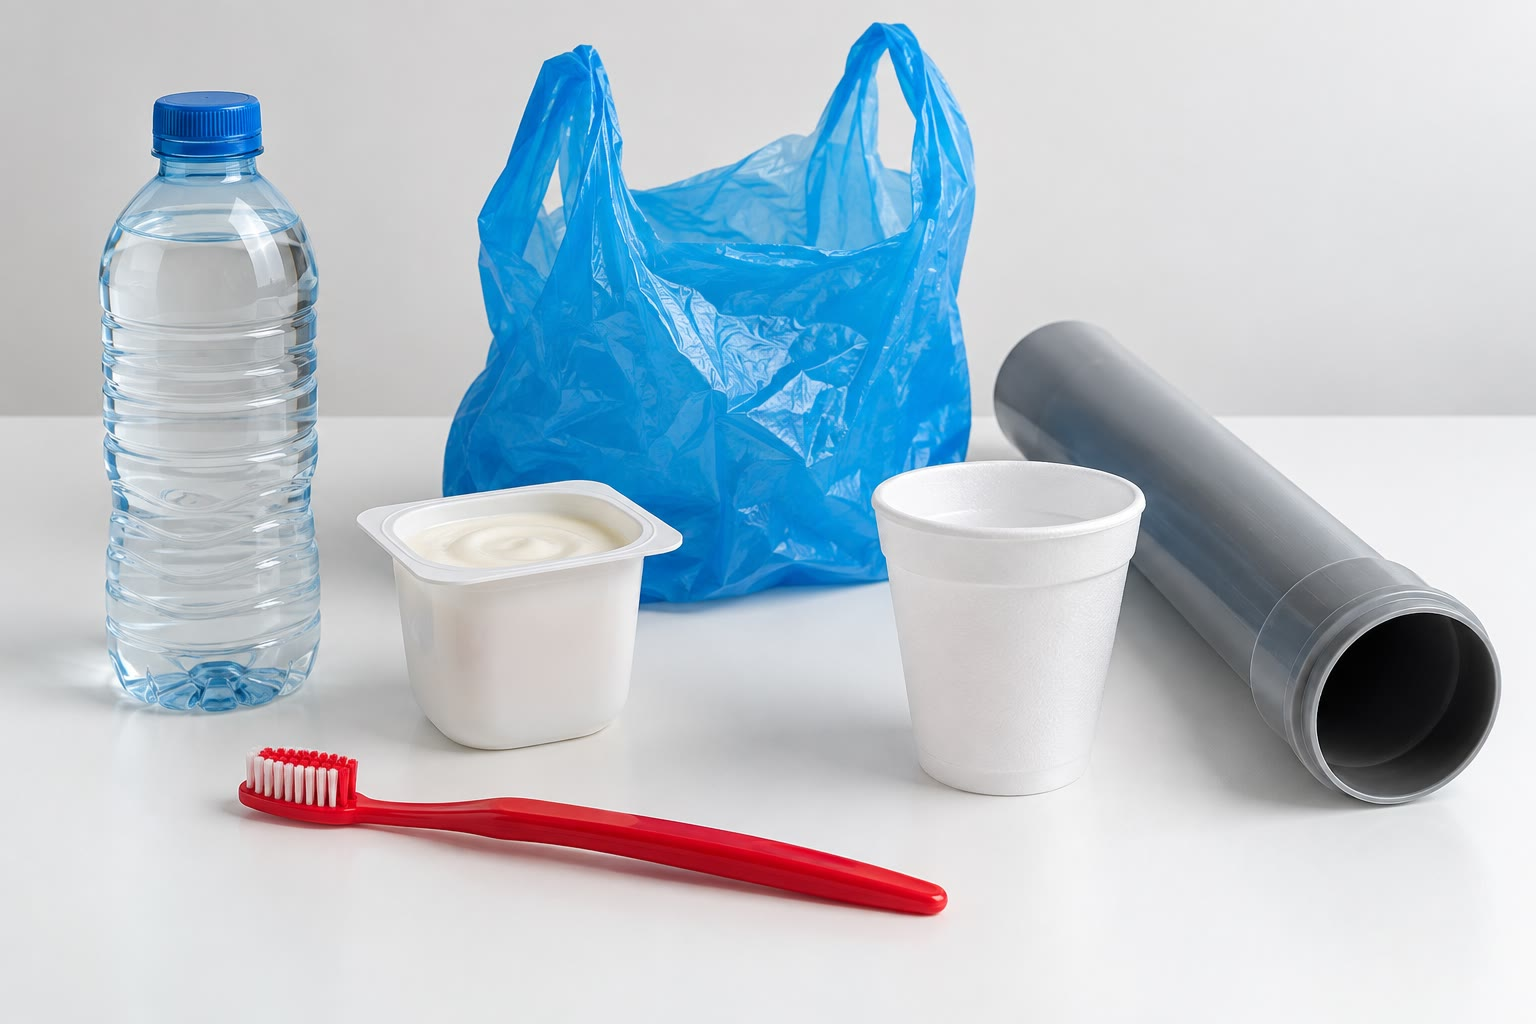
\includegraphics[width=0.55\linewidth]{images/book1/ai/g8-plastic-objects.jpg}

{\small रोज़मर्रा की \omterm{def:g8:plastics:plastic}{प्लास्टिक} वस्तुएँ: बोतल, डिब्बा, थैला, पाइप, कप,
टूथब्रश।}
\end{omfigure}

\section{प्राकृतिक, कृत्रिम और संश्लिष्ट सामग्रियाँ}

\begin{definition}[कृत्रिम और संश्लिष्ट सामग्रियाँ]\label{def:g8:plastics:artificial}
\omterm{def:g5:raw-materials-and-recycling:natural-material}{निर्मित सामग्रियों} में से \emph{कृत्रिम
सामग्री}\index{कृत्रिम सामग्री} किसी \omterm{def:g5:raw-materials-and-recycling:natural-material}{प्राकृतिक सामग्री} के रासायनिक
रूपांतरण से बनती है: लकड़ी के सेलुलोस से कागज़ और विस्कोस (एक कपड़ा)।
\emph{संश्लिष्ट सामग्री}\index{संश्लिष्ट सामग्री} रसायनज्ञों द्वारा बनाए
गए पदार्थों से बनती है, ज़्यादातर कच्चे तेल से, और प्रकृति में उसका कोई
समकक्ष नहीं होता: नाइलॉन, पॉलिएस्टर, \omterm{def:g8:plastics:plastic}{प्लास्टिक}।
\end{definition}

\begin{omfigure}
\begin{tikzpicture}[font=\small, level distance=1.5cm,
    box/.style={draw=omDef, fill=omDef!6, rounded corners=2pt, align=center,
      inner sep=4pt, text width=3.3cm},
    level 1/.style={sibling distance=6.4cm},
    level 2/.style={sibling distance=3.8cm},
    edge from parent/.style={draw, thick, omDef, ->}]
  \node[box] {सामग्रियाँ}
    child {node[box] {प्राकृतिक\\ \footnotesize सूत, ऊन, लकड़ी}}
    child {node[box] {निर्मित}
      child {node[box] {कृत्रिम\\ \footnotesize कागज़, विस्कोस}}
      child {node[box, draw=omProp, fill=omProp!6] {संश्लिष्ट\\ \footnotesize नाइलॉन,
        पॉलिएस्टर, प्लास्टिक}}};
\end{tikzpicture}

{\small प्राकृतिक, कृत्रिम और \omterm{def:g8:plastics:artificial}{संश्लिष्ट सामग्रियाँ}।}
\end{omfigure}

\section{प्लास्टिक क्या हैं}

\begin{definition}[प्लास्टिक]\label{def:g8:plastics:plastic}
\emph{प्लास्टिक}\index{प्लास्टिक} बहुत लंबे \omterm{def:g7:atoms-and-molecules:molecule}{अणुओं} से बनी एक \omterm{def:g8:plastics:artificial}{संश्लिष्ट सामग्री}
है, जिसे साँचे में ढालकर आकार दिया जा सकता है --- ज़्यादातर तब, जब वह गरम
और नरम हो --- और जो ठंडी होने पर अपना आकार बनाए रखती है। ज़्यादातर प्लास्टिक
कच्चे तेल या प्राकृतिक गैस से बनते हैं।
\end{definition}

\begin{remark}[बहुत लंबे अणु]\label{rem:g8:plastics:long}
पानी के एक \omterm{def:g7:atoms-and-molecules:molecule}{अणु} में तीन \omterm{def:g7:atoms-and-molecules:atom}{परमाणु} होते हैं; किसी \omterm{def:g8:plastics:plastic}{प्लास्टिक} के एक \omterm{def:g7:atoms-and-molecules:molecule}{अणु} में दसियों
हज़ार \omterm{def:g7:atoms-and-molecules:atom}{परमाणु} हो सकते हैं, जो एक लंबी श्रृंखला में जुड़े होते हैं, एक जैसे मनकों
की माला की तरह। ऐसी श्रृंखलाएँ कैसे बनती हैं, यह इस पुस्तक के अंत के एक अध्याय
का विषय है।
\end{remark}

\begin{omfigure}
\begin{tikzpicture}[font=\small]
  \foreach \k in {0,...,17} {
    \pgfmathsetmacro\x{0.62*\k}
    \pgfmathsetmacro\y{0.35*sin(40*\k)}
    \shade[ball color=omDef!50] (\x,\y) circle (0.22);
  }
  \node[anchor=west] at (11.2,0) {\dots};
  \node[anchor=north, align=center] at (5.3,-0.6) {हज़ारों एक जैसी इकाइयों की श्रृंखला};
\end{tikzpicture}

{\small यह एक चित्र है, मॉडल नहीं: \omterm{def:g8:plastics:plastic}{प्लास्टिक} का \omterm{def:g7:atoms-and-molecules:molecule}{अणु} एक जैसी इकाइयों की
बहुत लंबी श्रृंखला है।}
\end{omfigure}

\begin{history}[बैकेलाइट, 1907]
पहला पूरी तरह संश्लिष्ट \omterm{def:g8:plastics:plastic}{प्लास्टिक} 1907 में रसायनज्ञ लियो बैकलैंड ने बनाया,
कोलतार से मिलने वाले फ़ीनॉल और फ़ॉर्मेल्डिहाइड से। कठोर, गहरे रंग का और
ऊष्मा-रोधी बैकेलाइट टेलीफ़ोनों, रेडियो और बिजली के स्विचों की सामग्री बन गया।
1930 के दशक में नाइलॉन आया, फिर दूसरे विश्वयुद्ध के बाद बोतलों और थैलों
के \omterm{def:g8:plastics:plastic}{प्लास्टिक}।
\end{history}

\begin{omfigure}
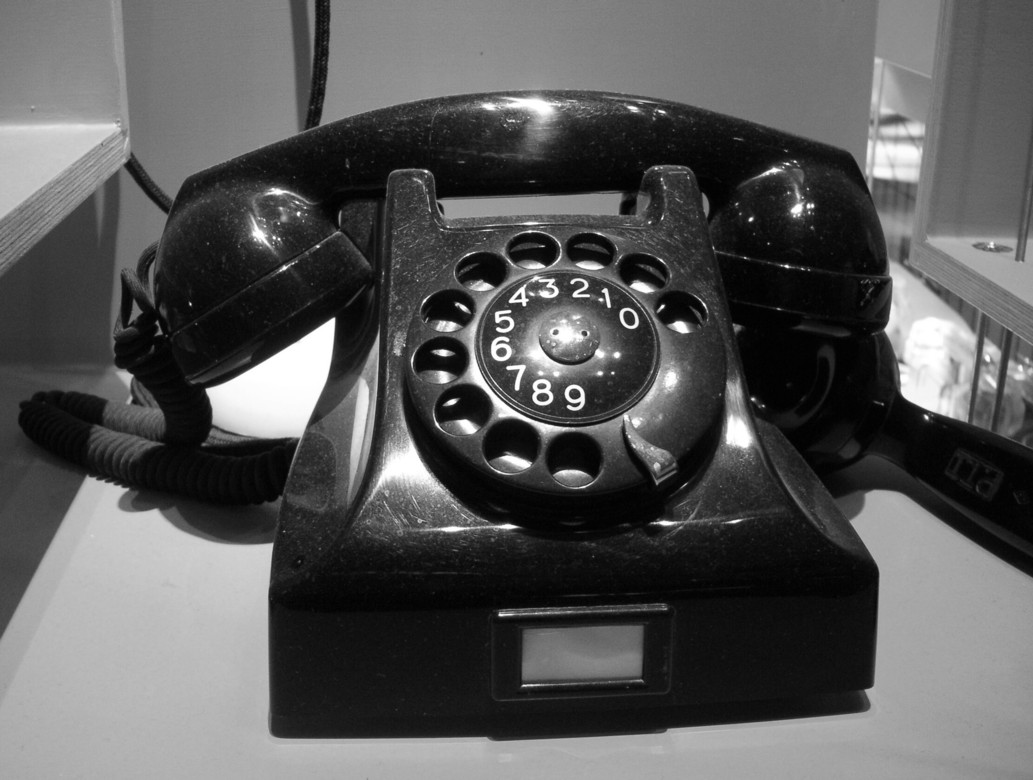
\includegraphics[width=0.42\linewidth]{images/book1/bakelite-telephone.jpg}

{\small 1947 का बैकेलाइट टेलीफ़ोन। फ़ोटो: होल्गर एलगार्ड,
CC BY-SA 3.0।}
\end{omfigure}

\section{मुख्य प्लास्टिक और उनके कोड}

\begin{definition}[रेज़िन पहचान कोड]\label{def:g8:plastics:code}
\emph{रेज़िन पहचान कोड}\index{रेज़िन पहचान कोड}
1 से 7 तक की एक संख्या है, जो किसी \omterm{def:g8:plastics:plastic}{प्लास्टिक} वस्तु पर तीरों के एक त्रिभुज के
भीतर छपी होती है और बताती है कि वस्तु किस \omterm{def:g8:plastics:plastic}{प्लास्टिक} से बनी है, ताकि उसे
\omterm{def:g5:raw-materials-and-recycling:recycling}{पुनर्चक्रण} के लिए छाँटा जा सके। त्रिभुज का अर्थ यह नहीं कि वस्तु का \omterm{def:g5:raw-materials-and-recycling:recycling}{पुनर्चक्रण}
होगा ही।
\end{definition}

\begin{proposition}[सात कोड]\label{prop:g8:plastics:codes}
कोड, हर \omterm{def:g8:plastics:plastic}{प्लास्टिक} के सबसे आम उपयोगों के साथ:
\begin{center}
\small
\begin{tabular}{cll}
\hline
कोड & \omterm{def:g8:plastics:plastic}{प्लास्टिक} & विशिष्ट वस्तुएँ \\
\hline
1 & PET, पॉलिएथिलीन टेरेफ़्थेलेट & पानी और सोडा की बोतलें, फ़्लीस के रेशे \\
2 & HDPE, उच्च घनत्व पॉलिएथिलीन & दूध और शैम्पू की बोतलें, ढक्कन \\
3 & PVC, पॉलिविनाइल क्लोराइड & पाइप, खिड़कियों के चौखटे, केबल \\
4 & LDPE, निम्न घनत्व पॉलिएथिलीन & थैले, पन्नियाँ \\
5 & PP, पॉलिप्रोपिलीन & दही के डिब्बे, बोतलों के ढक्कन, कारों के बंपर \\
6 & PS, पॉलिस्टाइरीन & फ़ोम के कप और ट्रे, सीडी के डिब्बे \\
7 & अन्य \omterm{def:g8:plastics:plastic}{प्लास्टिक} & \omterm{def:g6:pure-substances-and-mixtures:mixture}{मिश्रण}, बहुपरती पैकिंग \\
\hline
\end{tabular}
\end{center}
\end{proposition}

\begin{omfigure}
\begin{tikzpicture}[font=\small]
  \foreach \n/\lab in {1/PET, 2/HDPE, 3/PVC, 4/LDPE, 5/PP, 6/PS, 7/अन्य} {
    \begin{scope}[xshift=(\n-1)*2.1cm]
      \foreach \a in {90,210,330} {
        \pgfmathsetmacro\b{\a+120}
        \draw[omDef, line width=1.1pt, ->, >={Stealth[length=4pt]}]
          ($(\a:0.75)!0.14!(\b:0.75)$) -- ($(\a:0.75)!0.86!(\b:0.75)$);
      }
      \node[font=\bfseries] at (0,-0.05) {\n};
      \node[anchor=north, font=\footnotesize] at (0,-0.8) {\lab};
    \end{scope}
  }
\end{tikzpicture}

{\small सात \omterm{def:g8:plastics:code}{रेज़िन पहचान कोड}, हर एक अपने \omterm{def:g8:plastics:plastic}{प्लास्टिक} के संक्षिप्त
नाम के साथ।}
\end{omfigure}

\section{थर्मोप्लास्टिक और थर्मोसेट}

\begin{definition}[थर्मोप्लास्टिक और थर्मोसेट]\label{def:g8:plastics:thermoplastic}
\emph{थर्मोप्लास्टिक}\index{थर्मोप्लास्टिक} हर बार गरम करने पर नरम हो जाता
है और ठंडा होने पर फिर सख़्त हो जाता है: उसे बार-बार पिघलाकर फिर से ढाला जा
सकता है (PET, पॉलिएथिलीन, PVC, पॉलिप्रोपिलीन, पॉलिस्टाइरीन)।
\emph{थर्मोसेट}\index{थर्मोसेट} पहली बार गरम करके ढालने पर हमेशा के लिए
जम जाता है: दोबारा गरम करने पर वह नरम नहीं होता बल्कि झुलस जाता है (बैकेलाइट,
गोंदों और नावों के ढाँचों की रेज़िनें)।
\end{definition}

\begin{remark}[किनका पुनर्चक्रण हो सकता है]\label{rem:g8:plastics:which}
\omterm{def:g8:plastics:thermoplastic}{थर्मोप्लास्टिक} को पिघलाकर फिर से ढाला जा सकता है: इन्हीं \omterm{def:g8:plastics:plastic}{प्लास्टिकों} का \omterm{def:g5:raw-materials-and-recycling:recycling}{पुनर्चक्रण}
करके नई वस्तुएँ बनाई जाती हैं। \omterm{def:g8:plastics:thermoplastic}{थर्मोसेट} को फिर से पिघलाया नहीं जा सकता।
\end{remark}

\section{पर्यावरण में प्लास्टिक}

\begin{proposition}[प्लास्टिक टिके रहते हैं]\label{prop:g8:plastics:last}
% ledger: plastics:use-2019, plastics:waste-2019, plastics:recycled-share-2019
2019 में दुनिया ने लगभग 46 करोड़ टन \omterm{def:g8:plastics:plastic}{प्लास्टिक} का उपयोग किया और लगभग
35.3 करोड़ टन \omterm{def:g8:plastics:plastic}{प्लास्टिक} कचरा फेंका; उपयोग हुए \omterm{def:g8:plastics:plastic}{प्लास्टिक} में पुनर्चक्रित
\omterm{def:g8:plastics:plastic}{प्लास्टिक} केवल लगभग \qty{6}{\percent} था। \omterm{def:g8:plastics:plastic}{प्लास्टिक} सड़ते नहीं:
प्रकृति में वे छोटे से छोटे टुकड़ों, यानी सूक्ष्म-प्लास्टिक, में टूटते जाते हैं,
जो नदियों, महासागरों, मिट्टी और जंतुओं के शरीर में पाए जाते हैं।
\end{proposition}

\begin{omfigure}
\begin{minipage}[t]{0.48\linewidth}\centering
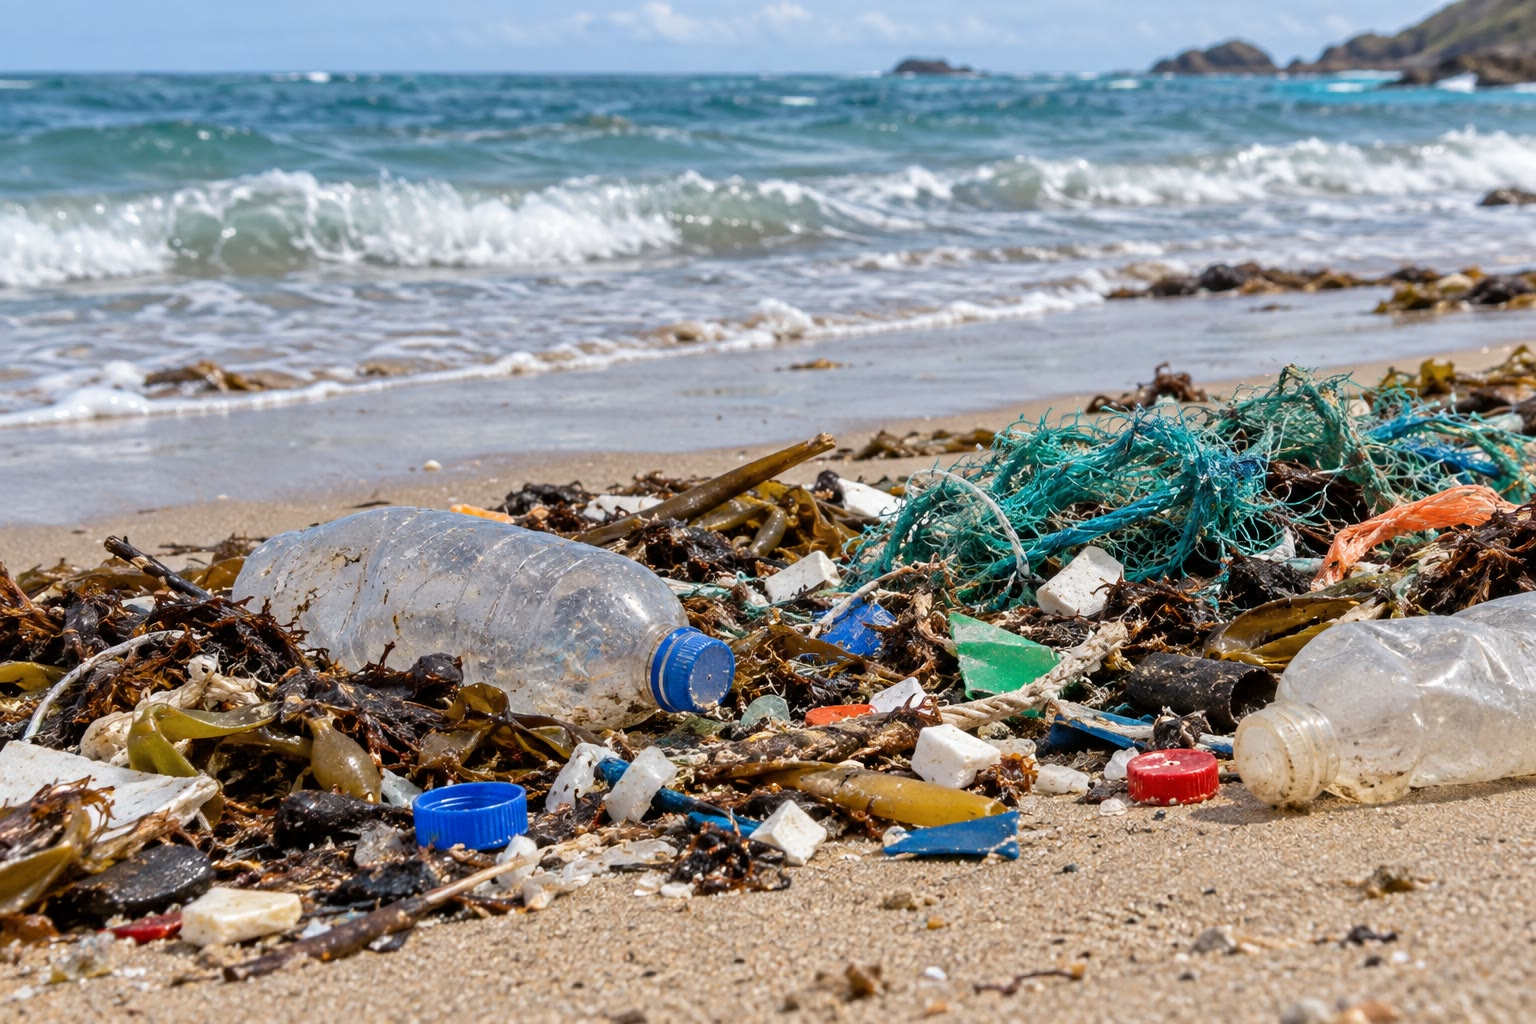
\includegraphics[width=\linewidth,height=4.6cm,keepaspectratio]{images/book1/ai/g8-beach-litter.jpg}

{\small समुद्र-तट पर बहकर आया \omterm{def:g8:plastics:plastic}{प्लास्टिक} कचरा।}
\end{minipage}\hfill
\begin{minipage}[t]{0.48\linewidth}\centering
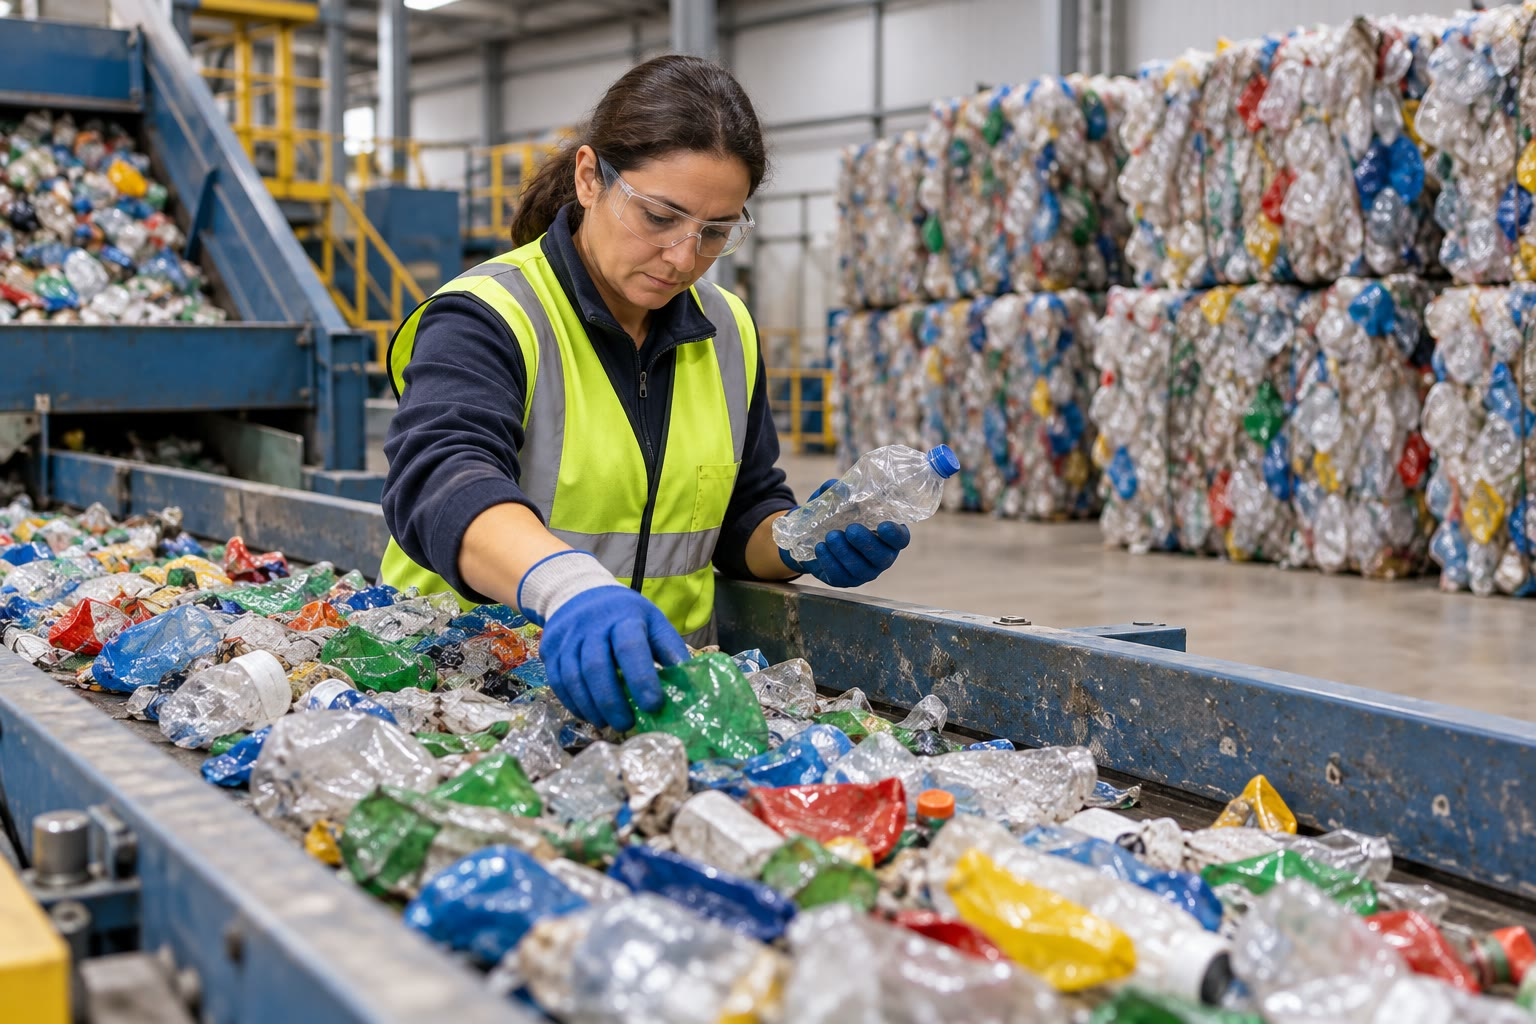
\includegraphics[width=\linewidth,height=4.6cm,keepaspectratio]{images/book1/ai/g8-sorting-line.jpg}

{\small \omterm{def:g8:plastics:plastic}{प्लास्टिक} \omterm{def:g5:raw-materials-and-recycling:recycling}{पुनर्चक्रण} संयंत्र की छँटाई लाइन।}
\end{minipage}
\end{omfigure}

\begin{remark}[प्लास्टिक जलाना]\label{rem:g8:plastics:burning}
\omterm{def:g8:plastics:plastic}{प्लास्टिक} \omterm{def:g4:what-a-fire-needs:burning}{जलते} हैं, और पूरी तरह \omterm{def:g4:what-a-fire-needs:burning}{जलने} पर कार्बन डाइऑक्साइड बनाते हैं।
पर बगीचे की आग में \omterm{def:g4:what-a-fire-needs:burning}{जलाने} पर वे अपूर्ण रूप से \omterm{def:g4:what-a-fire-needs:burning}{जलते} हैं और कालिख,
कार्बन मोनोऑक्साइड और दूसरे हानिकारक पदार्थ छोड़ते हैं; क्लोरीन वाला PVC
हाइड्रोजन क्लोराइड छोड़ता है, जो एक संक्षारक गैस है। \omterm{def:g8:plastics:plastic}{प्लास्टिक} कचरा केवल ऐसे
भस्मकों में \omterm{def:g4:what-a-fire-needs:burning}{जलाया} जाता है जो उनके धुएँ को साफ़ करने के लिए बने हों।
\end{remark}

\section{अभ्यास}

\begin{exercise}[$\star$]\label{exo:g8:plastics:1}
प्राकृतिक, कृत्रिम या संश्लिष्ट? सूत, नाइलॉन, कागज़, ऊन,
पॉलिस्टाइरीन, विस्कोस।
\end{exercise}

\begin{exercise}[$\star$]\label{exo:g8:plastics:2}
ज़्यादातर \omterm{def:g8:plastics:plastic}{प्लास्टिक} किस कच्चे माल से बनते हैं?
\end{exercise}

\begin{exercise}[$\star$]\label{exo:g8:plastics:3}
किस \omterm{def:g8:plastics:plastic}{प्लास्टिक} का कोड 1 है? उससे बनी एक वस्तु बताओ।
\end{exercise}

\begin{exercise}[$\star$]\label{exo:g8:plastics:4}
\omterm{def:g8:plastics:thermoplastic}{थर्मोप्लास्टिक} और \omterm{def:g8:plastics:thermoplastic}{थर्मोसेट} में क्या अंतर है?
\end{exercise}

\begin{exercise}[$\star\star$]\label{exo:g8:plastics:5}
दही के एक डिब्बे पर कोड 5 है। उसके \omterm{def:g8:plastics:plastic}{प्लास्टिक} का नाम बताओ, और बताओ कि
क्या सिद्धांत रूप में उसे पिघलाकर फिर से ढाला जा सकता है।
\end{exercise}

\begin{exercise}[$\star\star$]\label{exo:g8:plastics:6}
किसी वस्तु पर तीरों के त्रिभुज का अर्थ यह क्यों नहीं है कि उस वस्तु का
\omterm{def:g5:raw-materials-and-recycling:recycling}{पुनर्चक्रण} होगा?
\end{exercise}

\begin{exercise}[$\star\star$]\label{exo:g8:plastics:7}
कड़ाही का हत्था अक्सर \omterm{def:g8:plastics:thermoplastic}{थर्मोप्लास्टिक} के बजाय \omterm{def:g8:plastics:thermoplastic}{थर्मोसेट} से क्यों बनाया
जाता है?
\end{exercise}

\begin{exercise}[$\star\star$]\label{exo:g8:plastics:8}
इस अध्याय के 2019 के आँकड़ों से बताओ कि उस वर्ष उपयोग हुए \omterm{def:g8:plastics:plastic}{प्लास्टिक} का
कितना प्रतिशत कचरा बना। निकटतम पूर्ण संख्या तक पूर्णांकित करो।
\end{exercise}

\begin{exercise}[$\star\star$]\label{exo:g8:plastics:9}
PVC को बगीचे की आग में कभी क्यों नहीं जलाना चाहिए?
\end{exercise}

\begin{exercise}[$\star\star$]\label{exo:g8:plastics:10}
एक विद्यालय वर्ष के 36 हफ़्तों तक हर हफ़्ते \qty{25}{g} की 300 बोतलें
इस्तेमाल करता है। एक वर्ष में यह कितना \omterm{def:g8:plastics:plastic}{प्लास्टिक} हुआ?
\end{exercise}

\begin{exercise}[$\star\star\star$]\label{exo:g8:plastics:11}
पॉलिएथिलीन केवल कार्बन और हाइड्रोजन से बना है। उसके \omterm{def:g8:combustion-and-fuels:complete}{पूर्ण दहन} के उत्पाद
लिखो। समझाओ कि उसे \omterm{def:g4:what-a-fire-needs:burning}{जलाने} से \omterm{def:g8:combustion-and-fuels:fossil}{जीवाश्म ईंधन} की तरह \omterm{def:g4:air-a-mixture-of-gases:air}{वायु} में कार्बन डाइऑक्साइड
क्यों जुड़ती है।
\end{exercise}

\begin{exercise}[$\star\star\star$]\label{exo:g8:plastics:12}
समझाओ कि समुद्र में खोई \omterm{def:g8:plastics:plastic}{प्लास्टिक} की एक बोतल वर्षों बाद किसी मछली के भीतर
सूक्ष्म-प्लास्टिक के रूप में कैसे पहुँच सकती है।
\end{exercise}

\section{समस्या: छँटाई लाइन}

\begin{problem}[{सप्ताहांत समस्या --- इस्तेमाल हुई बोतलों का एक टन, उनके
कोड, और संयंत्र से निकलने वाले प्लास्टिक के साफ़ टुकड़े}]
\label{pb:g8:plastics:1}
एक \omterm{def:g5:raw-materials-and-recycling:recycling}{पुनर्चक्रण} संयंत्र में इस्तेमाल हुई पेय की बोतलों के गट्ठर आते हैं। \qty{1}{t}
(\qty{1000}{kg}) के एक सामान्य गट्ठर में द्रव्यमान के अनुसार होते हैं:
\qty{80}{\percent} PET की बोतलों के ढाँचे, \qty{12}{\percent} ढक्कन (HDPE
और PP), \qty{5}{\percent} लेबल (PP की पन्नी) और \qty{3}{\percent} गंदगी
और बचा हुआ द्रव। मशीनें ढक्कनों और लेबलों को ढाँचों से अलग करती हैं, PET
को पीसकर छोटे टुकड़े (फ़्लेक) बनाए जाते हैं, और टुकड़ों को धोया जाता है; धुलाई
में PET का \qty{2.5}{\percent} खो जाता है। साफ़ टुकड़ों को पिघलाकर फ़्लीस
जैकेटों के रेशे काते जाते हैं।

\medskip
\noindent\textbf{भाग I --- \omterm{def:g8:plastics:plastic}{प्लास्टिक}।}
\begin{enumerate}
  \item बोतलों के ढाँचों पर कौन-सा कोड छपा है? ढक्कनों पर?
  \item ये \omterm{def:g8:plastics:plastic}{प्लास्टिक} प्राकृतिक हैं, कृत्रिम या संश्लिष्ट?
  \item क्या PET को पिघलाकर फिर से काता जा सकता है? इससे वह किस प्रकार का
        \omterm{def:g8:plastics:plastic}{प्लास्टिक} ठहरता है?
  \item PET को पिघलाने से पहले ढक्कनों और लेबलों को ढाँचों से अलग क्यों
        किया जाता है?
\end{enumerate}

\medskip
\noindent\textbf{भाग II --- गट्ठर।}
\begin{enumerate}[resume]
  \item एक गट्ठर में कितना PET है?
  \item कितने ढक्कन (द्रव्यमान में)? कितने लेबल?
  \item गट्ठर का कितना द्रव्यमान \omterm{def:g8:plastics:plastic}{प्लास्टिक} नहीं है?
  \item गट्ठर का कितना प्रतिशत \omterm{def:g8:plastics:plastic}{प्लास्टिक} है?
\end{enumerate}

\medskip
\noindent\textbf{भाग III --- टुकड़े।}
\begin{enumerate}[resume]
  \item धुलाई में कितना PET खो जाता है?
  \item एक फ़्लीस जैकेट के लिए \qty{0.39}{kg} PET रेशा चाहिए। उसे नए PET के
        बजाय टुकड़ों से बनाना बेहतर क्यों है?
  \item संयंत्र ढक्कनों और लेबलों का \omterm{def:g5:raw-materials-and-recycling:recycling}{पुनर्चक्रण} करने के बजाय उन्हें ऊष्मा के लिए
        जला सकता है। इससे \omterm{def:g4:air-a-mixture-of-gases:air}{वायु} में कौन-सी गैस जुड़ेगी, उसका नाम बताओ।
  \item एक गट्ठर से मिलने वाले साफ़ PET टुकड़ों का द्रव्यमान निकालो।
\end{enumerate}
\end{problem}
